%%%%%%%%%%%%%%%%%%%%%%%%%%%%%%%%%%%%%%%%%
% Stylish Article
% LaTeX Template
% Version 2.1 (1/10/15)
%
% This template has been downloaded from:
% http://www.LaTeXTemplates.com
%
% Original author:
% Mathias Legrand (legrand.mathias@gmail.com) 
% With extensive modifications by:
% Vel (vel@latextemplates.com)
%
% License:
% CC BY-NC-SA 3.0 (http://creativecommons.org/licenses/by-nc-sa/3.0/)
%
%%%%%%%%%%%%%%%%%%%%%%%%%%%%%%%%%%%%%%%%%

%----------------------------------------------------------------------------------------
%	PACKAGES AND OTHER DOCUMENT CONFIGURATIONS
%----------------------------------------------------------------------------------------

\documentclass[fleqn,10pt]{SelfArx} % Document font size and equations flushed left

\usepackage[english]{babel} % Specify a different language here - english by default

\usepackage{lipsum} % Required to insert dummy text. To be removed otherwise

%----------------------------------------------------------------------------------------
%	COLUMNS
%----------------------------------------------------------------------------------------

\setlength{\columnsep}{0.55cm} % Distance between the two columns of text
\setlength{\fboxrule}{0.75pt} % Width of the border around the abstract

%----------------------------------------------------------------------------------------
%	COLORS
%----------------------------------------------------------------------------------------

\definecolor{color1}{RGB}{0,0,90} % Color of the article title and sections
\definecolor{color2}{RGB}{0,20,20} % Color of the boxes behind the abstract and headings

%----------------------------------------------------------------------------------------
%	HYPERLINKS
%----------------------------------------------------------------------------------------

\usepackage{hyperref} % Required for hyperlinks
\hypersetup{hidelinks,colorlinks,breaklinks=true,urlcolor=color2,citecolor=color1,linkcolor=color1,bookmarksopen=false,pdftitle={Title},pdfauthor={Author}}

%----------------------------------------------------------------------------------------
%	ARTICLE INFORMATION
%----------------------------------------------------------------------------------------

\JournalInfo{Data Mining B565 Fall 2016} % Journal information
\Archive{} % Additional notes (e.g. copyright, DOI, review/research article)

\PaperTitle{Analysis and Prediction of House Prices for the City of Ames} % Article title

\Authors{Anusha Ramamurthy\textsuperscript{1}, Vandana Kolli\textsuperscript{2}} % Authors
\affiliation{\textsuperscript{1}\textit{ Data Science, School of Informatics and Computing, Indiana University, Bloomington, IN, USA}} % Author affiliation
\affiliation{\textsuperscript{2}\textit{ Computer Science, School of Informatics and Computing, Indiana University, Bloomington, IN, USA}} % Author affiliation
\affiliation{*\textbf{Corresponding author}: todo} % Corresponding author

\Keywords{house --- price --- prediction} % Keywords - if you don't want any simply remove all the text between the curly brackets
\newcommand{\keywordname}{Keywords} % Defines the keywords heading name

%----------------------------------------------------------------------------------------
%	ABSTRACT
%----------------------------------------------------------------------------------------

\Abstract{In this paper, we analyzed the house price based on multiple features using data mining algorithms. In order to select a prediction method different regression methods were explored and compared. The dataset we used describes the sale of individual residential property in Ames, Iowa from 2006 to 2010. We built models using linear regression, decision trees and random forests and compared their performances. The problem
	is how to reduce multiple features to a minimal number(feature extraction) that can completely predict the target price variable. The results show that data mining algorithms produces high prediction accuracy in house price analysis and prediction. }

%----------------------------------------------------------------------------------------

\begin{document}
	
	\flushbottom % Makes all text pages the same height
	
	\maketitle % Print the title and abstract box
	
	\tableofcontents % Print the contents section
	
	\thispagestyle{empty} % Removes page numbering from the first page
	
	%----------------------------------------------------------------------------------------
	%	ARTICLE CONTENTS
	%----------------------------------------------------------------------------------------
	
	\section{Introduction} % The \section*{} command stops section numbering
	
	\addcontentsline{toc}{section}{Introduction} % Adds this section to the table of contents
	
	\subsection{Problems in House Price Prediction}
	Real estate properties will always be a safe option of investment for a common person. It is an investment which does not decline in value rapidly. The rapidly growing real estate industry has become an important part of national economy. Problems such as rapid raise of house price, high vacancy ratio require the Government to institute industrial policies to help industry development. With the increase on the data, the analysts need to apply good tools and predict house prices to help consumers. There is a lot of house data available with different features like Lot Area, Street, neighborhood etc. The important thing is to find a efficient data analysis tool to transform the data into knowledge and information\cite{irb}.\\
	The data comprises of the multiple features of the house which can be considered by potential buyers , but it is impossible to provide an automated comparison on all the features as they are diverse. The diversity of features makes it challenging to predict correct market price. Feature Extraction is one of the biggest challenges faced with data having large feature set. The house predict
	
	
	\subsection{Data Minning on House Price prediction}
	Data mining is the process of understanding useful and structural patterns in data, thus referring to the overall procedure of information discovery from data. These data specific discoveries became popular in the domain of machine learning and artificial intelligence. Some of the most popular machine learning algorithm include - decision trees, linear regression, logistic regression, neural networks, random forests and so on. Each algorithm suits some problems better than others. Data mining techniques are used to extract knowledge from data using a different of methods that are divided in two groups: classification and regression. Classification learns to map, or classifies, an item in the data into one of several predefined classes while regressions maps the item to a continuous numerical prediction.
	
	Data mining draws inferences from data to understand the patterns of correlation among data values and to predict the future data values. By calculating the differences between the actual and predicted price as an error, we compare the results and accuracy of the predicated prices by the Decision Trees and Neural Networks algorithms. 
	
	\subsection{Interests and Motivation}
	TODO
	The consumers of the house price prediction can be - homeowners, investors, tax assessment department, insurers etc. These consumers should get an accurate prediction of the final price of house. It is interesting to learn based diverse features on the existing consumer data and predict accurate house prices for any new data.  
	
	\footnote{And some mathematics $\cos\pi=-1$ and $\alpha$ in the text.}.
	
	%------------------------------------------------
	
	\section{Background}
	
	\begin{figure*}[ht]\centering % Using \begin{figure*} makes the figure take up the entire width of the page
		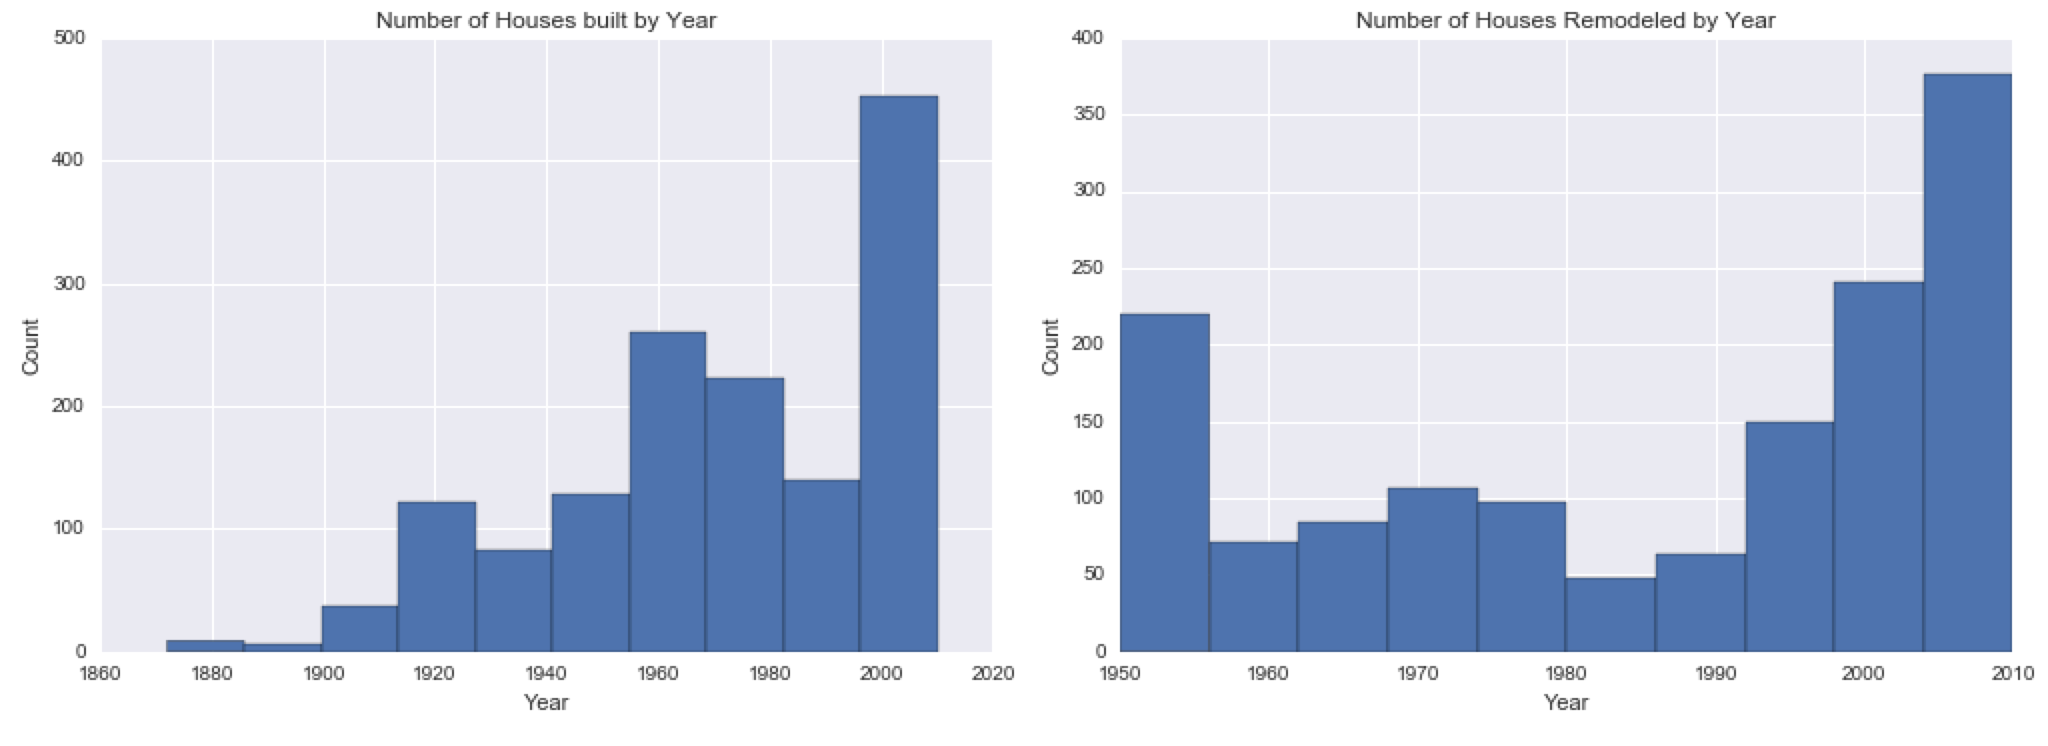
\includegraphics[width=\linewidth]{year}
		\caption{Count of Houses Built and Remodeled}
		\label{fig:year}
	\end{figure*}
	\begin{figure*}[ht]\centering % Using \begin{figure*} makes the figure take up the entire width of the page
		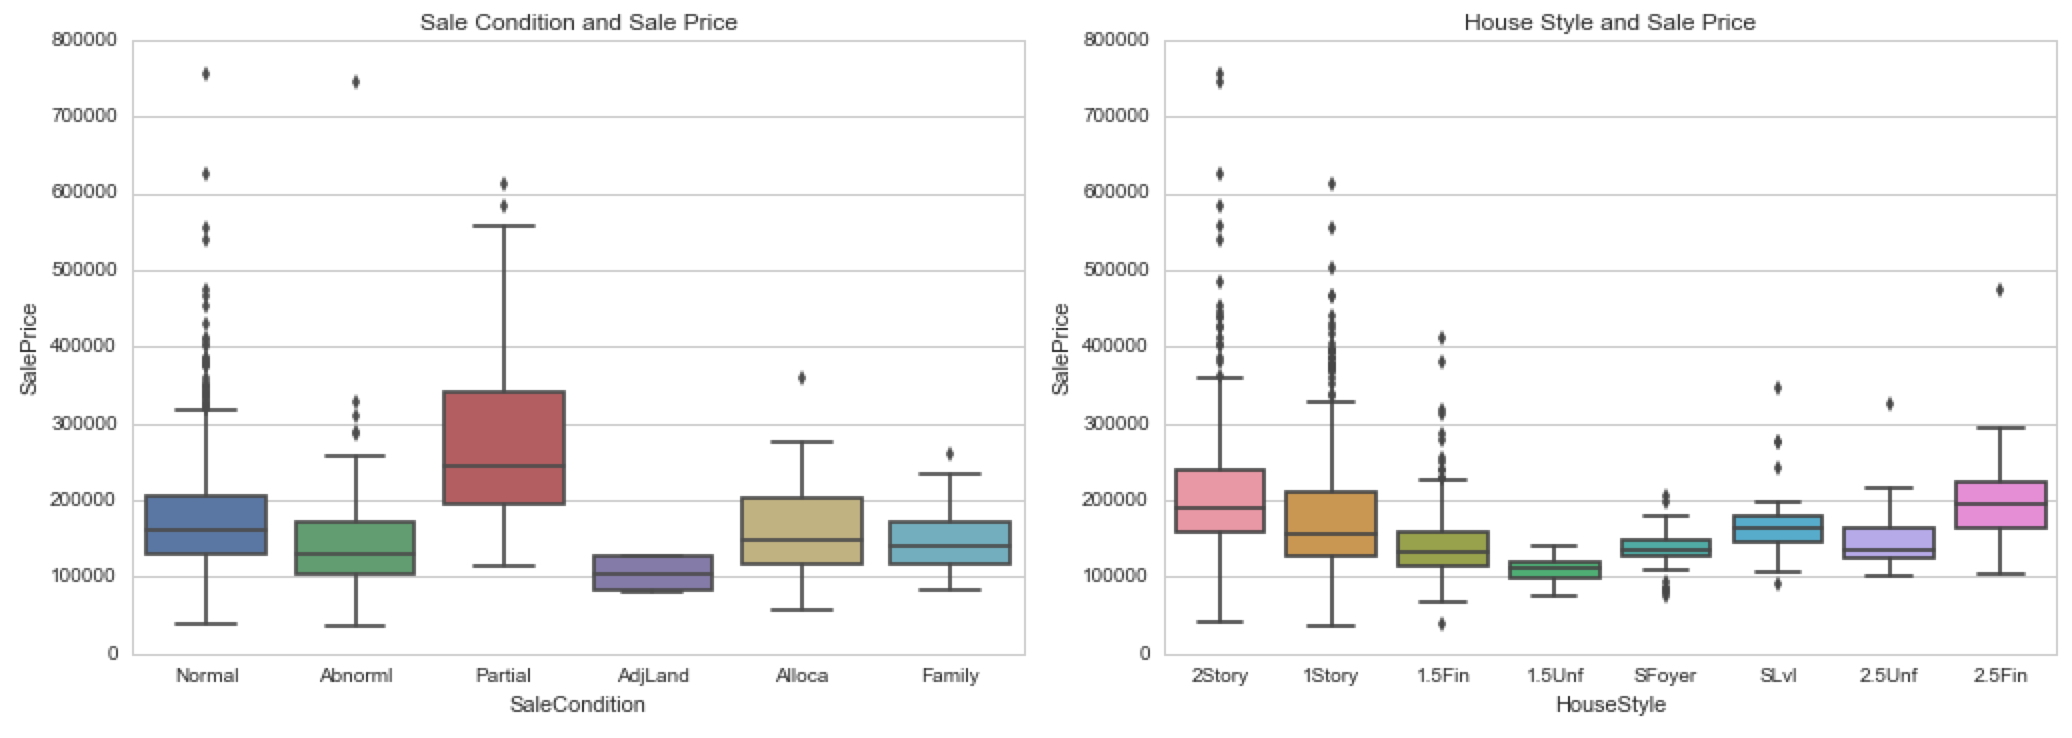
\includegraphics[width=\linewidth]{SalePrice}
		\caption{Distribution of Sale Price}
		\label{fig:SalePrice}
	\end{figure*}
	
	In this paper we used machine learning algorithms like linear regression, decision trees and neural networks to predict the house prices. Machine learning techniques can be divided into supervised and unsupervised. Our analysis takes into consideration the provided target variables in making predictions, thus it is supervised. In this section we will discuss about these techniques in detail.
	\subsection{Linear Regression}
	A Regression Model defines three types of regression models: linear, polynomial, and logistic regression. Linear regression, the most widely used of all statistical techniques, allows to summarize and study relations between two continuous variables\cite{stat}. It attempts to model the relationship between these two variables by fitting a linear equation to observed data. \\
	Let $Y$ be the target value which we need to predict.\\
	Let $X$ be the independent variables from which target is predicted, then\\
	The linear regression line has an equation of the form:
	\[ $Y = a + bX$\]
	Mos common method to fit a regression line is the method of least squares which calculates the best fitting line for observed data by minimizing the sum of squares of the vertical deviations from each data point to the line. 
	
	\subsection{Decision Trees}
	A decision tree builds regression or classification models in the form of a tree structure. The tree includes root node, branches and leaf nodes. Each internal node denotes a test on an attribute, each branch denotes the outcome of a test and each leaf node holds a class label. Decision trees can handle both categorical and numerical data. \\
	Different algorithms and impurity measures are used for building a Decision Tree. In our analysis we have used CART (Classification and Regression Tree) algorithm. In our paper since we are dealing with prediction of a continuous  variable(price), the decision tree is called regression tree.\\
	\textbf{Gini Index}\\
	It measures the inequality among values of a frequency distribution. Gini index of 0 means perfect equality(where all values are same) and Gini index of 1 means maximum inequality among values. The impurity(or purity) measure used in building decision tree in CART is called GINI index.
	\[Gini Index = 1 - \sum_{j}p_j^2 \]
	
	\subsection{Neural Networks}
	Artificial Neural network is a computing system made up of a number of simple, highly interconnected processing elements, which process information by their dynamic state response to external inputs.
	%------------------------------------------------
	
	\section{Data Analysis}
	
	\subsection{Data Description}
	The dataset consisted of information about 2919 houses in the City of Ames, Iowa, United States of America. These houses were split into two sets, one  with information about 1460 houses, each has 81 attributes, 79 of them describe various aspects and quality of the house, two others being the ID, identification number for each house and the other is an attribute we wish to predict, the Sale Price of the house. Among the 79, we found 23 attributes to be nominal, 23 to be ordinal, 14 were discrete and 19 continuous set of values \cite{dataset}.\\
	
	\begin{table}[hbt]
		\caption{Table of Attribute Types}
		\centering
		\begin{tabular}{llr}
			\cmidrule(r){1-2}
			Attribute Type & Count \\
			\midrule
			Nominal & 23 \\
			Ordinal & 23 \\
			Discrete & 14 \\
			Continous & 19
		\end{tabular}
		\label{tab:label}
	\end{table}
	
	All the continuous variables are the dimensions measured in square feet, for example the size of the lot, the basement area, the size of the living area and so on. The 14 discrete variables are the count of the various commodities present in the house, for example the count of the bedrooms, bathrooms and so on. The 46 categorical variables describe aspects like the quality of the house, fireplace pool and so on, as well as information about the neighborhood the house belongs to. Hence we couldn't eliminate missing values as there would be no row available.\\
	
	\subsection{Exploratory Analysis}
	We begin our analysis by checking for duplicates, a check of Id values showed 1460 unique observations. We found that among the 81 attributes, 19 of them had missing values. An initial exploratory analysis of the 62 attributes that had no missing values revealed some interesting insights. \\
	
	A thousand four hundred and sixty houses were sold in just four years. The year 2009 appears to have seen the highest number of sales with 338 houses sold. Around 551 of the house's appear to have been built between 1999 and 2010, while 909 of the houses that were sold between 2006 and 2010,  were built between 1870 and 1989. Around 178 of these houses were remodeled in the year 1950, 20 of these were built in the year 1920. Clearly the year a house was built seems to be a factor in the sale of a house, but only further investigations can say if it was an advantage or not. Does the age of house make it more attractive to a buyer? It appears hard to say. From the graphs, most of the houses appear to have been remodeled during 1950-1955 and 2000-2010. \\
	
	It also appears that amongst most forms of Sale, Normal conditions of the sale appear to have fetched the highest price. But, houses that were not complete when last assessed also seem to fetch a higher price(Partial Condition). In fact looking at the distribution it appears that these fetched a broader range of prices than most other form of Sale Conditions. It also appears that Two story houses fetched the highest price as well as having Two and one-half story and One story houses fetched the next best prices. In both graphs we see houses that fetched a very high price, these may be possible outliers. 
	
	\subsection{Missing Values}
	A large part of analysis depends on the amount of data we have. A large volume of data allows our  data mining algorithms to train better and eventually reduce the margin of error. With the current data set we found 19 attributes containing missing values. Every row of our observations had at least one attribute with a missing value. 
	
	\begin{table}[hbt]
		\caption{Table of Missing Values}
		\centering
		\begin{tabular}{llr}
			\cmidrule(r){1-2}
			Attribute Name &  Type & Missing \\
			\midrule
			Electrical & Nominal & 1 \\
			MasVnrType & Nominal & 8 \\
			MasVnrArea & Continous & 8 \\
			BsmtQual & Nominal & 37 \\
			BsmtCond & Nominal & 37 \\
			BsmtExposure & Nominal & 38 \\
			BsmtFinType1 & Nominal & 37 \\
			BsmtFinType2 & Nominal & 38 \\
			GarageType & Nominal & 81 \\
			GarageYrBlt & Continuous & 81 \\ 
			GarageFinish & Nominal & 81 \\
			GarageQual & Nominal & 81 \\
			GarageCond & Nominal & 81 \\
			LotFrontage & Continuous & 259 \\
			FireplaceQu & Nominal & 690 \\
			Fence & Nominal & 1179 \\
			Alley & Nominal & 1369 \\
			MiscFeature & Nominal & 1406 \\
			PoolQC & Nominal & 1453 \\	
		\end{tabular}
		\label{tab:label}
	\end{table}

	\subsection{Replacing Missing Values}
	

	\section{Problem}
	TODO
	
	
	\section{Experiments Data}
	TODO
	The model proposed in this paper was trained on a very
	large and diverse dataset. In this section we describe the
	details of the dataset. In addition, we also discuss the details
	of the various standard techniques that have been used for
	the problem, with which the performance of the model was
	compared. The results of the various techniques are given
	in the next section. The data set describes the sale of individual residential property in Ames, Iowa from 2006 to 2010. The data set contains a large number of explanatory variables (23 nominal, 23 ordinal, 14 discrete, and 20 continuous) involved in assessing home
	values.\\
	Operating System: \\
	Python Version: \\
	Any other tools used \\
	
	
	
	
	\section{Results}
	We first trained our system using 80 of train data and then tested on rest of 20 of the train data. 
	\section{Summary conclusion}
	\section{Future Work}
	In future we are planning to work with random forests. In a random forest, each node is split using the best among a subset of predictors randomly chosen at that node. This somewhat counter intuitive strategy turns out to perform very well compared to many other classifiers.
	\section{Appendix}
	%------------------------------------------------
	\phantomsection
	\section*{Acknowledgments} % The \section*{} command stops section numbering
	
	\addcontentsline{toc}{section}{Acknowledgments} % Adds this section to the table of contents
	
	So long and thanks for all the fish \cite{Figueredo:2009dg}.
	
	%----------------------------------------------------------------------------------------
	%	REFERENCE LIST
	%----------------------------------------------------------------------------------------
	\phantomsection
	\bibliographystyle{unsrt}
	\bibliography{/Users/aramamurthy/Downloads/Github/Kaggle-HPAR/references.bib}
	%----------------------------------------------------------------------------------------
	
\end{document}